\documentclass[conference]{IEEEtran}

% *** GRAPHICS RELATED PACKAGES ***
%
\ifCLASSINFOpdf
  \usepackage{graphicx}
  % declare the path(s) where your graphic files are
  \graphicspath{{./figures/}}
  \DeclareGraphicsExtensions{.pdf,.jpeg,.png,.jpg}
\else
  \usepackage{graphicx}
  % declare the path(s) where your graphic files are
  \graphicspath{{./figures/}}
  \DeclareGraphicsExtensions{.eps}
\fi

\usepackage{multirow}
\usepackage{float}


\newcommand{\FigRef}[1]{Fig.~\ref{fig:#1}}
\newcommand{\TabRef}[1]{Table~\ref{tab:#1}}


\begin{document}
% paper title
% can use linebreaks \\ within to get better formatting as desired
% Do not put math or special symbols in the title.
\title{On Video Background Subtraction Using Robust PCA Methods}

% author names and affiliations
\author{
\IEEEauthorblockN{Richard Al-Bayaty}
\IEEEauthorblockA{School of Electrical and Computer Engineering\\
University of Florida\\
Gainesville, FL 32611\\
Email: ralbayaty@ufl.edu}
\\
}

\maketitle


\begin{abstract}
%Abstract - A paragraph that summarizes the problem and the results.
There are many application areas for background subtraction techniques, some of which being object tracking, image segmentation, human pose estimation, and change detection. Of the many ways by which background subtraction is performed, a robustification of the well known Principal Component Analysis (PCA) has been frequently adopted. In background detection, it is assumed that the dataset is composed of a low rank matrix and a sparse outlier matrix. This robust PCA (RPCA) method allows for the decomposition of a dataset into both the low rank and the sparse outlier portions, which models the background and the foreground respectively.

 
\end{abstract}
\hfill

\begin{IEEEkeywords}
Background subtraction, foreground detection, robust PCA, video processing.
\end{IEEEkeywords}

\section{Introduction}
%	Introduction - Sets the context, describes the problem, and describes your solution.

In video analysis, it is often desired to parse video streams into both a foreground and background. The background of a video stream contains objects and scenery which do not necessarily change swiftly, while the foreground is taken to be objects which move more independently and regularly than the background. An example of this would be a surveillance camera pointed towards a parking lot. The parking lot, street lights, any grass or shrubbery as well as the painted lines should be considered as the background, while the foreground would be the cars, people, animals, and other objects as they come in and out of the lot. One of the methods used for performing foreground detection (or background detection) is to model the video as a dataset which can be decomposed as $ X = L + S $, where X is the vectorized frames from the video scene into a data matrix, L is a low rank matrix which represents the aforementioned background and S is the sparse outlier matrix representing the foreground. Other methods incorporate an additional matrix, E, which aims to model additional noise from either the process itself or measurements. The optimization problem for the robust version of PCA (Principal Component Pursuit) is formulated by Candes \cite{Candes} as:

\begin{equation} \label{eq:PCP}
\begin{array}{rrclcl}
\textrm{arg} \displaystyle \min_{L,S} & \multicolumn{3}{l}{||L||_* + \lambda ||S||_1} \\
\textrm{s.t.} & X & = & L + S \\
\end{array}
\end{equation}

The PCP framework allows for a convenient model towards background subtraction in that the total scene can be regarded as being composed of the L and S matrices. This work aims to highlight some of the more recent background subtraction algorithms developed using RPCA.


% Paper organization: Section I, Section II, etc...
The rest of this paper is organized as follows: Section II covers the work related to this project and gives an overview of some of the currently used RPCA algorithms for background subtraction, Section III covers the qualitative and quantitative analysis, Section IV discusses the experiments performed including visualizations of experiment results, and Section V concludes the study with a summary and recommendations for future work.

\section{Related Work}
%	Related work - Describes representative works related to your work, and summarizes the pros and cons of each work.
This work is comprised mainly of a brief introduction to the topic area as well as a superficial explanation of  some of the algorithms used to accomplish the background subtraction task. More thorough investigations of methodologies and a rigourous attempt at utlizing quantitative measures for algorithm comparisons are performed by both Bouwmans \cite{RPCAreview} and Sobral \cite{Sobral}. The following sub sections elaborate on some non-RPCA methods as well as introduce the RPCA methods that are evaluated in Section IV.

\subsection{Non-RPCA methods}
There are other methods besides those modeled with RPCA that have been used successfully in previous years. Some of the techniques include Static Frame Difference, where a frame from the video sequence without foreground noise is chosen as being the background and subsequence frames are differenced from this image to produce the foreground. This technique is sensitive to both illumination and dynamic scenes, so an advancement to this framework was to use the previous frame instead of a static image for differencing. This technique was coined further Frame Difference. 

Another methodology for this problem is to use statistical models such as Gaussian Mixture Models (GMM) to represent each pixel and calculate the likelihood of a particular pixel as being background/foreground for a given pixel value. This model can be updated in an online fashion using an expectation maximization algorithm. 

Neural and neuro-fuzzy network models have also been used with great success. Each pixel is deemed as belonging to background/foreground by a Bayesian classifier while the background model is learned through the neural network.

\subsection{Fast Principal Component Pursuit (FPCP) \cite{FPCP}}
In fast principal component pursuit, a minor variation to the original PCP optimization problem is introduced and an alternating minimization technique is proposed. This variation is shown in equation \ref{eq:FPCP}.

\begin{equation} \label{eq:FPCP}
\begin{array}{rrclcl}
\textrm{arg} \displaystyle \min_{L,S} & \multicolumn{3}{l}{\frac{1}{2}||L+S-D||_F + \lambda ||S||_1} \\
\textrm{s.t.} & rank(L) & = & t \\
\end{array}
\end{equation}

The alternating minimizations shown in equations \ref{eq:FPCP1} and \ref{eq:FPCP2} allow for an expedient solution recovery.

\begin{equation} \label{eq:FPCP1}
L_{k+1} = \textrm{arg} \displaystyle \min_{L} ||L+S_k-D||_F \;\;\; \textrm{s.t.} \; rank(L) = t
\end{equation}
\begin{equation} \label{eq:FPCP2}
S_{k+1} = \textrm{arg} \displaystyle \min_{S} ||L_{k+1}+S-D||_F  + \lambda ||S||_1
\end{equation}

The solution to equation \ref{eq:FPCP1} comes from computing a t-component Singular Value Decomposition (SVD) of $D- S_k$. Solving equation \ref{eq:FPCP2} is performed with an element-wise shrinkage, shrink($D-L_{k+1},\lambda$). 




\subsection{Go Decomposition (GoDec) \cite{GoDec}}
The GoDec algorithm expands upon the traditional PCP framework by presuming that the L and S are not exactly recoverable due to Gaussian noise corruption of the form  $ X = L + S + G$, and thus incorporates an L2 minimization as the optimal estimator for a model with additive Gaussian noise constraining the rank and the cardinality of L and S as shown in equation \ref{eq:GoDec}. To further approximate and boost the speed of this algorithm, the authors proposed replacing the SVD solving method in lieu of a bilateral random projection based low-rank approximation to the Naive GoDec algorithm.

\begin{equation} \label{eq:GoDec}
\begin{array}{rrclcl}
\displaystyle \min_{L,S} & \multicolumn{3}{l}{||X-L-S||_F^2} \\
\textrm{s.t.} & rank(L) & \leq & r \\
                   & card(C) & \leq & k \\
\end{array}
\end{equation}

\subsection{Semi-Soft GoDec (SSGoDec) \cite{GoDec}}
While GoDec applies a hard threshold to both the singular values of the low rank matrix L and the sparse entries of the matrix S, the Semi-Soft variant allows for a soft thresholding to the values in S. This adaptation provides a strength in that the parameter k to control the cardinality of S is now automatically driven by the soft thresholding parameter $\tau$. In GoDec, if one chose the value of k to be too large then S could absorb some of the noise introduced by the additive noise matrix G. This soft-thresholding also allows for a boost to the computation speed of the algorithm.

\subsection{Reinforced Robust Principal Component Pursuit ($R^2$-PCP)}
To handle the need to model outliers in both the principal component space as well as the orthogonal component space of the transformed subspace, $R^2$-PCP offers a data model as follows in equation \ref{eq:R^2-PCP1} :

\begin{equation} \label{eq:R^2-PCP1}
\begin{array}{rrclcl}
X =  B + O + (1\mu^T + S)V_\perp^T + E & \\
 \textrm{with} \;\; rank(B) \leq r \\
\end{array}
\end{equation}

B is low rank, O is the sparse principal component outlier matrix, E is an additive noise matrix, and the remaining term, $(1\mu^T + S)V_\perp^T$, is the orthogonal space outlier matrix.This problem can be formulated as equation \ref{eq:R^2-PCP2}, where $P_O(O;\lambda_O)$ and $P_S(S;\lambda_S)$ are general sparsity penalties with $\lambda_O$ and $\lambda_S$ as regularization parameters.

\begin{equation} \label{eq:R^2-PCP2}
\begin{array}{rrclcl}
\displaystyle \min_{V_\perp, \mu, O, S} & \multicolumn{3}{l}{\frac{1}{2}||(X-O)V_\perp - 1\mu^T - S||_F^2 + P_O(O;\lambda_O) + P_S(S;\lambda_S) } \\
\textrm{s.t.} & V_\perp^TV_\perp & = & I \\
\end{array}
\end{equation}

Given $\mu, O, S$, equation \ref{eq:R^2-PCP2} is optimized for $V_\perp$ as an unconstrained problem on the Stiefel manifold.


\section{Description}
%	Description - One or more sections that describes the problem and your approach to the solution in detail.
A vast amount of background subtraction datasets are available to test different algorithm performance. The dataset used for comparing these algorithms comes from the ChangeDetection.NET (CDNET) 2014 dataset \cite{changedetection}. A subset of the video sequences CDNET2014 were used, namely the baseline highway and the baseline pedestrians. This dataset contains many video sequences to test the robustness of algorithms in many ways, such as with night vision videos, panning/tilting/zooming, dynamic backgrounds, and bad weather. Since the function of this work is aimed at introducing the topic and algorithms, using the baseline videos were sufficient. 

Each video sequence, highway and pedestrian, are split into frames, converted to grayscale to remove two-thirds the values, and vectorized to construct an n by p matrix, X, where n is the number of frames and p is $m*n$ (frame height times frame width). This matrix is then fed to the selected RPCA algorithms to obtain outputs consisting of a background (L), a foreground (S), and a hard-thresholded version of the foreground (O) to highlight the nature of the foreground outliers. To compare results quantitatively, the peak signal-to-noise ratio (PSNR) was used between the provided ground truth after being hard-thresholded (to remove intermediary gray levels) and the outputs of the algorithms. The algorithm with the highest PSNR is deemed to have reproduced the best foreground for the given video sequence.



\section{Evaluation}
%	Evaluation - A section that quantitatively evaluates your ideas.
The code used to run FPCP, GoDec, and SSGoDec was obtained from ``Low-Rank and Sparse Tools for Background Modeling and Subtraction in Videos'' library created by Andrews Sobral \cite{LRSLibrary}. The code for $R^2$-PCP was made available through the Multimedia, Communications, and Networking Lab from the dissertation of Dr. Shijie Li.

Tables \ref{tab:runtime} and \ref{tab:PSNR} show the run times of the algorithms and the PSNR as compared to the ground truth, respectively. The GoDec algorithm stood out as being the fastest for both datasets, while the performance of the SSGoDec was superior.


\begin{table}[h]
\renewcommand{\arraystretch}{1.2}
\caption{Algorithm run times (seconds)} \label{tab:runtime}
\centering
\begin{tabular}{|c|c|c|c|c|}
    \hline
      & FPCP & GoDec & SSGoDec & $R^2$-PCP\\
    \hline
% Data goes here
    Highway & 249.7573 & 81.3508 & 865.2944 & Unk\\
    \hline
    Pedestrian & 89.2926 & 45.1151 & 608.7915 & Unk\\
    \hline
\end{tabular}
\end{table}

\begin{table}[h]
\renewcommand{\arraystretch}{1.2}
\caption{Algorithm PSNR (decibels)} \label{tab:PSNR}
\centering
\begin{tabular}{|c|c|c|c|c|}
    \hline
      & FPCP & GoDec & SSGoDec & $R^2$-PCP\\
    \hline
% Data goes here
    Highway & 10.9708 & 7.4582 & 11.6149 & Unk\\
    \hline
    Pedestrian & 15.7586 & 15.7529 & 15.9369 & Unk\\
    \hline
\end{tabular}
\end{table}



In Figures \ref{fig:output1_1} and \ref{fig:output1_2}, the ground truth for a single frame of the two video sequences are shown on the left-most column, while the remaining columns show the outputs for that particular frame in the three algorithms that provided outputs. It is difficult to make a qualitative comparison in these results since they are seemingly very similar. A comparison between the input video sequence frame and the resultant background and foreground from the algorithms is shown in Figures \ref{fig:output2_1} and \ref{fig:output2_2}.

\begin{figure}[H] 
\begin{center} 
\noindent
  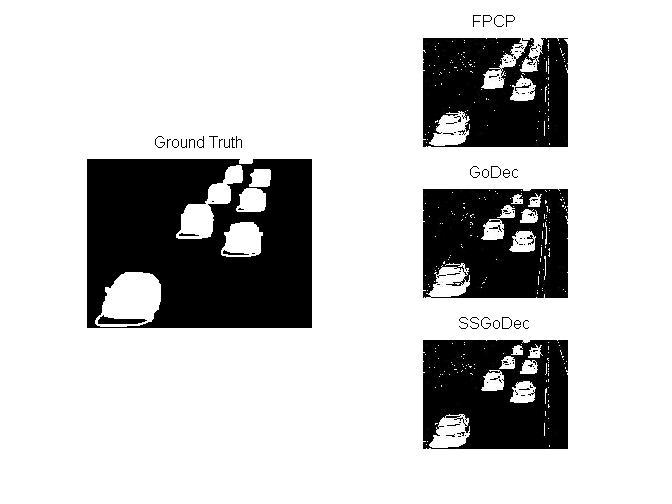
\includegraphics[width=.8\columnwidth]{highway} 
  \caption{Comparison to ground truth for highway sequence} \label{fig:output1_1}
  \noindent
  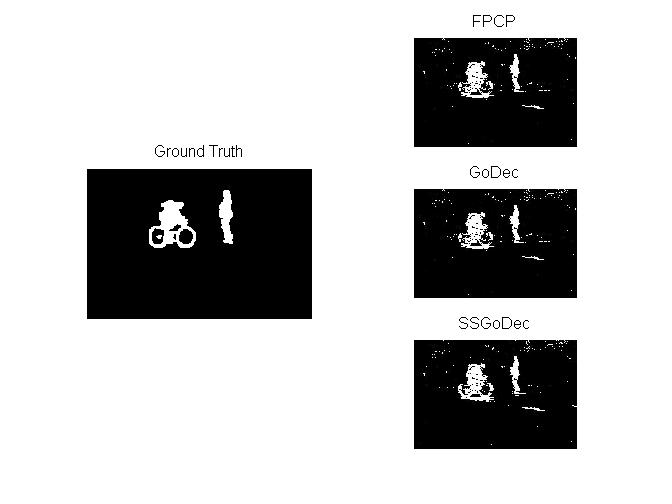
\includegraphics[width=.8\columnwidth]{pedestrians}
  \caption{Comparison to ground truth for pedestrian sequence}  \label{fig:output1_2}
\end{center}
\end{figure}

\begin{figure}[H]
\begin{center}  
\noindent
  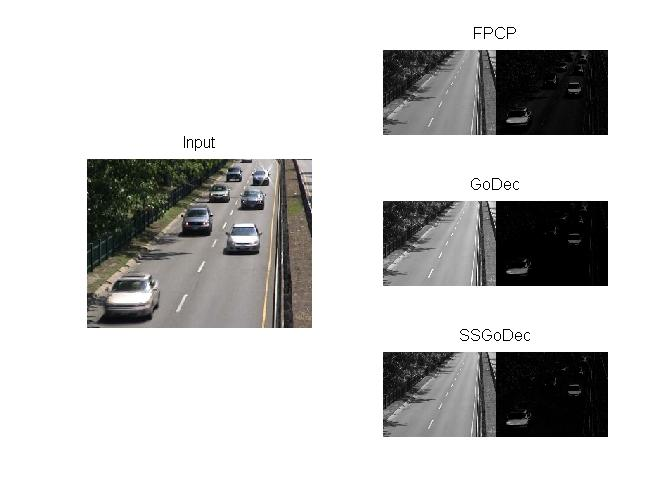
\includegraphics[width=.8\columnwidth]{highway2}
  \caption{The input compared to the L and S outputs for highway} \label{fig:output2_1}
  \noindent
  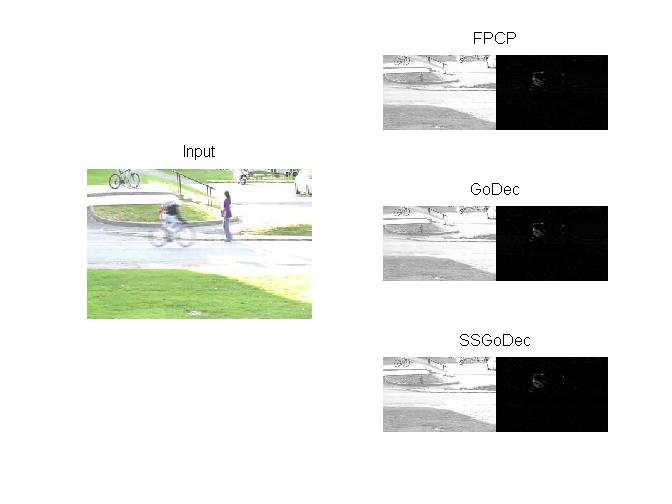
\includegraphics[width=.8\columnwidth]{pedestrians2}
  \caption{The input compared to the L and S outputs for pedestrians} \label{fig:output2_2}
\end{center}
\end{figure}



\section{Conclusion}
%	Summary and Conclusions - Summarize what you did and what interesting things you learned from the project.
The task of splitting a video sequence into two separate sequences, a background and foreground, using methodologies from PCP was introduced. A handful of currently used algorithms were explained and run on a reputable dataset in order to make comparisons between the algorithms' run times and their output quality. It was shown for one run of the algorithms that GoDec succeeded in the fastest run time while SSGoDec  achieved best PSNR for foreground detection, given the ground truth of the foreground provided in the CDNET 2014 dataset. Unfortunately, the novel and new algorithm $R^2$-PCP was not capable of processing the datasets in any acceptable amount of time due to the nature of the optimization problem and the computing limitations for this experimentation. In order to test the performance of this algorithm, a more compact and fast solver must be developed or found to be implemented for use with large datasets such as the ones used in this experimentation.

\newpage


% references section

% can use a bibliography generated by BibTeX as a .bbl file
% BibTeX documentation can be easily obtained at:
% http://www.ctan.org/tex-archive/biblio/bibtex/contrib/doc/
% The IEEEtran BibTeX style support page is at:
% http://www.michaelshell.org/tex/ieeetran/bibtex/
%\bibliographystyle{IEEEtran}
% argument is your BibTeX string definitions and bibliography database(s)
%\bibliography{IEEEabrv,../bib/paper}
%
% <OR> manually copy in the resultant .bbl file
% set second argument of \begin to the number of references
% (used to reserve space for the reference number labels box)
\begin{thebibliography}{7}

\bibitem{Candes}
Candès, Emmanuel J., Xiaodong Li, Yi Ma, and John Wright. ``Robust principal component analysis?." Journal of the ACM (JACM) 58, no. 3 (2011): 11.

\bibitem{RPCAreview}
Thierry Bouwmans, El Hadi Zahzah, ``Robust PCA via Principal Component Pursuit: A review for a comparative evaluation in video surveillance'', Computer Vision and Image Understanding, Volume 122, May 2014, Pages 22-34, ISSN 1077-3142, http://dx.doi.org/10.1016/j.cviu.2013.11.009.
%(http://www.sciencedirect.com/science/article/pii/S1077314213002294)
%Abstract: Abstract
%Foreground detection is the first step in video surveillance system to detect moving objects. Recent research on subspace estimation by sparse representation and rank minimization represents a nice framework to separate moving objects from the background. Robust Principal Component Analysis (RPCA) solved via Principal Component Pursuit decomposes a data matrix A in two components such that A = L + S , where L is a low-rank matrix and S is a sparse noise matrix. The background sequence is then modeled by a low-rank subspace that can gradually change over time, while the moving foreground objects constitute the correlated sparse outliers. To date, many efforts have been made to develop Principal Component Pursuit (PCP) methods with reduced computational cost that perform visually well in foreground detection. However, no current algorithm seems to emerge and to be able to simultaneously address all the key challenges that accompany real-world videos. This is due, in part, to the absence of a rigorous quantitative evaluation with synthetic and realistic large-scale dataset with accurate ground truth providing a balanced coverage of the range of challenges present in the real world. In this context, this work aims to initiate a rigorous and comprehensive review of RPCA-PCP based methods for testing and ranking existing algorithms for foreground detection. For this, we first review the recent developments in the field of RPCA solved via Principal Component Pursuit. Furthermore, we investigate how these methods are solved and if incremental algorithms and real-time implementations can be achieved for foreground detection. Finally, experimental results on the Background Models Challenge (BMC) dataset which contains different synthetic and real datasets show the comparative performance of these recent methods.
%Keywords: Foreground detection; Robust principal component analysis; Principal Component Pursuit

\bibitem{Sobral}
Andrews Sobral, Antoine Vacavant, ``A comprehensive review of background subtraction algorithms evaluated with synthetic and real videos'', Computer Vision and Image Understanding, Volume 122, May 2014, Pages 4-21, ISSN 1077-3142, http://dx.doi.org/10.1016/j.cviu.2013.12.005.
%(http://www.sciencedirect.com/science/article/pii/S1077314213002361)
%Abstract: Abstract
%Background subtraction (BS) is a crucial step in many computer vision systems, as it is first applied to detect moving objects within a video stream. Many algorithms have been designed to segment the foreground objects from the background of a sequence. In this article, we propose to use the BMC (Background Models Challenge) dataset, and to compare the 29 methods implemented in the BGSLibrary. From this large set of various BG methods, we have conducted a relevant experimental analysis to evaluate both their robustness and their practical performance in terms of processor/memory requirements.
%Keywords: Background subtraction; Motion detection; Foreground segmentation

\bibitem{FPCP}
Rodriguez, P.; Wohlberg, B., ``Fast principal component pursuit via alternating minimization," Image Processing (ICIP), 2013 20th IEEE International Conference on , vol., no., pp.69,73, 15-18 Sept. 2013
doi: 10.1109/ICIP.2013.6738015
%Abstract: We propose a simple alternating minimization algorithm for solving a minor variation on the original Principal Component Pursuit (PCP) functional. In computational experiments in the video background modeling problem, the proposed algorithm is able to deliver a consistent sparse approximation even after the first outer loop, (taking approximately 12 seconds for a 640 × 480 × 400 color test video) which is approximately an order of magnitude faster than Inexact ALM to construct a sparse component of the same quality.
%keywords: {approximation theory;image colour analysis;minimisation;principal component analysis;video signal processing;PCP functional;alternating minimization;color test video;principal component pursuit functional;sparse approximation;video background modeling problem;Approximation algorithms;Approximation methods;Image color analysis;Minimization;Robustness;Streaming media;Video sequences;Principal Component Pursuit;Video Background Modeling},
%URL: http://ieeexplore.ieee.org/stamp/stamp.jsp?tp=&arnumber=6738015&isnumber=6737993


\bibitem{GoDec}
Zhou, Tianyi, and Dacheng Tao. ``Godec: Randomized low-rank \& sparse matrix decomposition in noisy case." In Proceedings of the 28th International Conference on Machine Learning (ICML-11), pp. 33-40. 2011.

\bibitem{changedetection}
Y. Wang, P.-M. Jodoin, F. Porikli, J. Konrad, Y. Benezeth, and P. Ishwar, ``CDnet 2014: An Expanded Change Detection Benchmark Dataset'', 
in Proc. IEEE Workshop on Change Detection (CDW-2014) at CVPR-2014, pp. 387-394. 2014
(http://www.changedetection.net)


\bibitem{LRSLibrary}
Sobral, A. and Baker, C. G. and Bouwmans, T. and Zahzah, E, ``Incremental and Multi-feature Tensor Subspace Learning applied for Background Modeling and Subtraction", International Conference on Image Analysis and Recognition (ICIAR'14), Oct. 2014
%    url          = "https://github.com/andrewssobral/imtsl"



\end{thebibliography}




\end{document}



%Instructions for Preparing Your Project Reports
%•	The length of a report must be no more than 10 pages.

%•	Reports must include the following parts:
%o	Project title and your name
%o	Abstract - A paragraph that summarizes the problem and the results.
%o	Introduction - Sets the context, describes the problem, and describes your solution.
%o	Description - One or more sections that describes the problem and your approach to the solution in detail.
%o	Evaluation - A section that quantitatively evaluates your ideas.
%o	Related work - Describes representative works related to your work, and summarizes the pros and cons of each work.
%o	Summary and Conclusions - Summarize what you did and what interesting things you learned from the project.
%o	Reference list

%Criteria Used for Grading Your Project Report
%1.	Quality. The value of a paper is a function of the innate character or degree of excellence of the work described. Was the work performed, or the study made with a high degree of thoroughness? Was high engineering skill demonstrated? Is an experiment described which has a high degree of elegance? Or, on the other hand, is the work described pretty much of a run-of-the-mill nature? 
%2.	Presentation. The value of the paper is a function of the ease with which the reader can determine what the author is trying to present. Regardless of the other criteria, a paper is not good unless the material is presented clearly and effectively. Is the paper well written? Is the meaning of the author clear? Are the tables, charts and figures clear? Is their meaning readily apparent? Is the information presented in the paper complete? At the same time, is the paper concise?
%3.	(Bonus) Originality. The value of a paper is a function of the degree to which it presents new or novel technical material. Does the paper present results previously unknown? Does it push forward the frontiers of knowledge? Does it present new methods for solving old problems or new viewpoints on old problems? Or, on the other hand, is it a re-hash of information already known?
%4.	(Bonus) Contribution. The value of a paper is a function of the degree to which it represents an overall contribution to the advancement of the art. This is different from originality. A paper may be highly original, but may be concerned with a very minor, or even insignificant, matter or problem. On the other hand, a paper may make a great contribution by collecting and analyzing known data and facts and pointing out their significance. Or, a fine exposition of a known, but obscure or complex, phenomenon or theory or system or operating technique may be a very real contribution to the art. Obviously, a paper may well score highly on both originality and contribution. Perhaps a significant question is, will the engineer who reads the paper be able to practice his profession more effectively because of having read it?

